\documentclass[a4paper, 11pt]{article}

%% Language and font encodings
\usepackage[english]{babel}
\usepackage[T1]{fontenc}

%% Sets page size and margins
\usepackage{geometry}
\geometry{
  includeheadfoot,
  margin = 2.54cm
}

%% Useful packages
\usepackage{amsmath}
\usepackage{amssymb}
\usepackage{bbm}
\usepackage{graphicx}
\usepackage{array}
\usepackage{hyperref}
\usepackage{booktabs}
\usepackage{minted}
\usepackage{float}
\usepackage{caption, subcaption}
\usepackage{csquotes}
% \usepackage{todonotes}
\usepackage{bm}

\renewcommand{\vec}[1]{\mathbf{#1}}
\newcommand{\0}{\phantom{0}}
\newcommand{\norm}[1]{\left\lVert#1\right\rVert_2}
\newcommand{\onenorm}[1]{\left\lVert#1\right\rVert_1}
\newcommand{\abs}[1]{\left|#1\right|}
\newcommand*{\vertbar}{\rule[-1ex]{0.5pt}{2.5ex}}
\newcommand*{\horzbar}{\rule[.5ex]{2.5ex}{0.5pt}}

\usepackage{tikz}
\usetikzlibrary{matrix,chains,positioning,decorations.pathreplacing,arrows}

\usepackage[backend = biber, style = ieee]{biblatex}
% If you want to break on URL numbers
\setcounter{biburlnumpenalty}{9000}
% If you want to break on URL lower case letters
\setcounter{biburllcpenalty}{9000}
% If you want to break on URL UPPER CASE letters
\setcounter{biburlucpenalty}{9000}
\AtEveryBibitem{\ifentrytype{misc}{}{\clearfield{url}}}
\AtEveryBibitem{\clearfield{issn}}
\AtEveryBibitem{\clearfield{isbn}}
\AtEveryBibitem{\clearfield{month}}
\DeclareFieldFormat{url}{Available: \url{#1}}
\DeclareFieldFormat*{title}{#1}
\addbibresource{library.bib}

\usepackage[english, notuetoc]{packages/frontpage}
\usepackage{tabto}
\title{Digit recognition using Linear Algebra and Deep Learning}
\subtitle{2WH40 Bachelor End Project \\~\\ \small{Menno Hofst\'e\tabto*{7em} (0996144)\\ \texttt{m.l.hofste@student.tue.nl}}}

\author{Menno Hofst\'e\tabto*{7em} (0996144)}

\orderissuer{Michiel Hochstenbach}
\copyholder{}
\administrativeunit{Department of Mathematics and Computer Science}
\department{\textit{Center for Analysis, Scientific Computing and Applications (CASA)}}
\Address{Postbus 513, 5600 MB Eindhoven\\ The Netherlands}

% \includeonly{techniques/knn}

\begin{document}
\maketitle
\begin{abstract}\noindent
  Applications of digit and character recognition are everywhere.
  This paper explores three different ways to classify handwritten digits, which are \(k\)-nearest neighbour algorithm, singular value decomposition, and neural network. First, we illustrate the techniques by numerical examples. Fundamentals of these techniques are explained, and their computational complexities and accuracies are discussed.
  Finally, we conclude that the different properties of the methods makes them useful for different applications.
\end{abstract}
\newpage
\thispagestyle{empty}
\setcounter{page}{0}
\tableofcontents
\section{Introduction}\label{s:intro}
Applications of automatic digit and character recognition are everywhere. 
Examples are recognising street signs, digitising old documents, or searching for words that appear in a photograph. 
The potential in this field is enormous, and as such there is also a lot of research done in this area~\cite{Anthonissen, Savas2007, Ciresan2010, Cao2006}. 
The automatic classification of handwritten digits is often considered as a standard problem in pattern recognition, because many challenges of pattern recognition are present~\cite{Savas2007}.
The research done in this area led to a number of ways to solve this problem. 
This thesis will give an overview of some of those popular techniques and compare them.

To compare the various techniques, we used labelled images from a subset of the US Postal Service Database which was packaged with a book from Hastie et al~\cite{Hastie2009}. 
This data set is split up into 2 sets. 
There is a training set, which consists of a digit and an image representing that digit. 
This is the only set which the algorithms and models have complete access to. 
The other set is called a test set. 
This set also consists of a digit and an image representing that digit; however in this case the algorithms and models only have access to the images. 
This set is given as input after which a classification attempt is made by using the technique under consideration on the test set. 
Then the corresponding digit in the test set can be used to decide whether or not the classification is correct.

Each image in the data set has a dimension of 16 \(\times \) 16 and thus consists of 256 pixels.
The image is a black-and-white monochrome image, where each pixel has a certain gray-scale value between \(-1\) and \(1\) with a step size of \(5\cdot 10^{-4}\). 
In this paper the lowest pixel value in an image is chosen to be completely white and the highest pixel value black. 
This is merely a convention such that the black digits are displayed on a white background.

The following structure is present in the paper.
First, in Section~\ref{s:knn}, test images will be compared with the training images with the \(k\)-nearest neighbour algorithm.
Secondly, in Section~\ref{s:svd_all}, test images are classified on their distance to subspaces spanned by the training images for a particular number.
Finally, in Section~\ref{s:neural_network}, images are classified through the use of a neural network model.

Section~\ref{s:knn} starts with the remark that each image can be represented by a point in a 256-dimensional space.
In this space each element of the vector corresponds to the brightness of a pixel, hence this space will be called the pixel space.
In this section, the similarity between two images is made more concrete.
Then the idea is to classify a test digit as the digit corresponding to the most similar digit.

Section~\ref{s:svd_all} exploits the fact that all training images for a particular number form a subspace. Using the singular value decomposition this space is represented in a more convenient way.
The idea is to classify a test digit as the digit corresponding to the closest subspace.

In Section~\ref{s:neural_network} we train a model on the training images in the hope that patterns pertaining to different images are extracted.
Test images are then given as input to the model, where the model can use the different patterns to recognise a digit.
Fundamental parts of a neural network will be explained with the use of a small example, after which it will be applied to the digit recognition problem.

Finally, we draw some conclusions in Section~\ref{s:conclusion}.
In the appendix the reader can find parts of the code created in MATLAB 2019a.

\section{\textit{k}-Nearest Neighbour (kNN)}\label{s:knn}
As mentioned in Section~\ref{s:intro} the test set is a subset of the data set from which both the label and the image may be used.
If an unlabelled image needs to be classified, we compare this image to each image in the training set and use the label of the most similar image.
The nearest neighbour algorithm is based on this idea~\cite{Cover1967}.

The nearest neighbour approach is very susceptible to outliers.
Imagine an image of a number zero that is written in such a way that it closely resembles a six, and that there are two other images of a six written in almost the same way as the zero.
Suppose you want to classify a six that most closely resembles the zero.
In that case all information of the other two images of a six are completely ignored, hence returning an incorrect result.
This particular problem can be avoided by looking at the three most similar images and choosing the most occurring one.
Looking at the three nearest neighbours is known as the \(k\)-nearest neighbour algorithm, where \(k = 3\).
For simplicity in the remainder of this section assumes that \(k = 1\) unless stated otherwise.

It is important to note that, disregarding the space and time constraints, one of the most difficult task for this particular technique is measuring similarity.
Section~\ref{s:knn:similarity} explores ways to relate different measures of similarity.
Accuracy is important, however for many applications the speed of the algorithm is also important and as a result the space and time complexity are the focus in Section~\ref{s:knn:complexity}.
In Section~\ref{s:knn:approximate} we try to optimise the technique further at the cost of accuracy.

\subsection{Similarity}\label{s:knn:similarity}
Before this technique can be used to solve the handwritten digit recognition problem, a measure of similarity needs to be established.
In mathematical terms, the pixel space needs to become a metric space.

\textbf{Definition~\cite{Bramwell2007}.} \textit{A metric space is a pair (X, d), where X is a set and d is a metric on X (or distance function on X), that is, a function defined on X\(\times \)X such that for all \(x, y, z\in X\) we have:
    \begin{itemize}
        \item \(d\) is real-valued, finite and non-negative.
        \item \(d(x, y) = 0\) if and only if \(x = y\).
        \item \(d(x,y) = d(y,x)\).
        \item \(d(x,y)\leq d(x,z) + d(z,y)\).
    \end{itemize}}

For the pixel space to become a metric space a suitable distance function needs to be defined.
A lot of research has been done in this area resulting in many different distances.
There are more generic distances such as the 1-norm and Euclidean distance, and there are more specialised distances.
Several distances useful for digit recognition are the Fuzzy Image Metric~(FIM)~\cite{JunliLi2002}, Generalized Hausdorff distance~\cite{Huttenlocher2003}, Tangent distance~\cite{Simard1992}, and IMage Euclidean Distance~(IMED)~\cite{LiweiWang2005}.

The FIM is primarily used in image quality assessment for image compression. The Generalized Hausdorff distance is very useful in comparing shapes in binary images.
The Tangent distance is developed particularly for digit recognition and takes various transformations into account.
IMED is similar to the more general Euclidean distance, however small perturbations result in a smaller difference~\cite{LiweiWang2005}.

First, we discuss the Euclidean distance and the 1-norm applied to the classification problem and their performance is measured.
After this, the Tangent distance will be inspected further as, according to Wang et al~\cite{LiweiWang2005}, it results in the highest accuracy among the distances relevant to digit recognition.

\subsubsection{Euclidean distance / 1-norm}
Both the Euclidean distance and the 1-norm are used to compare points in the pixel space.
Flattening an image consisting of 16 by 16 pixels results in a point in the pixel space. A visualisation of flattening a 3 by 3 image can be found in Figure~\ref{fig:flatten}.
\begin{figure}[H]
    \centering
    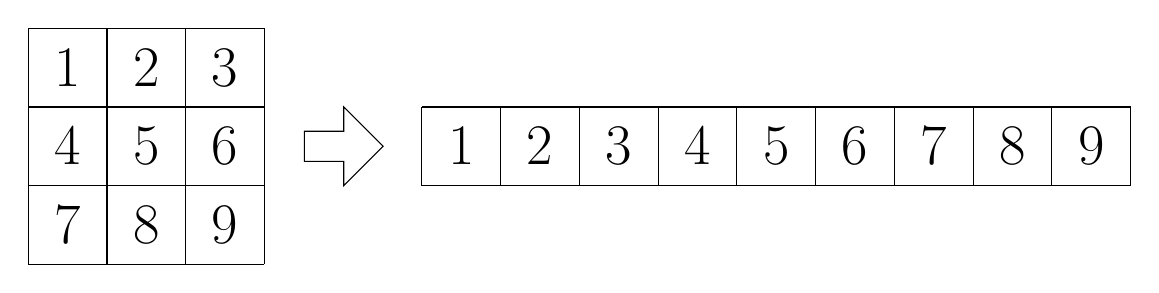
\begin{tikzpicture}
        \usetikzlibrary{shapes.arrows}

        % grid left
        \draw[step=1] (0,0) grid (3,3);
        \node at (.5, 2.5) {\huge 1};
        \node at (1.5, 2.5) {\huge 2};
        \node at (2.5, 2.5) {\huge 3};
        \node at (.5, 1.5) {\huge 4};
        \node at (1.5, 1.5) {\huge 5};
        \node at (2.5, 1.5) {\huge 6};
        \node at (.5, .5) {\huge 7};
        \node at (1.5, .5) {\huge 8};
        \node at (2.5, .5) {\huge 9};

        % arrow
        \node[draw, single arrow,
              minimum height=1cm, minimum width=1cm,
              single arrow head extend=2mm,
              anchor=west] at (3.5,1.5) {};

        % grid right
        \draw[step=1] (5,1) grid (14,2);
        \node at (5.5, 1.5) {\huge 1};
        \node at (6.5, 1.5) {\huge 2};
        \node at (7.5, 1.5) {\huge 3};
        \node at (8.5, 1.5) {\huge 4};
        \node at (9.5, 1.5) {\huge 5};
        \node at (10.5, 1.5) {\huge 6};
        \node at (11.5, 1.5) {\huge 7};
        \node at (12.5, 1.5) {\huge 8};
        \node at (13.5, 1.5) {\huge 9};
    \end{tikzpicture}
    \caption{Flattening, or reshaping, of a 3 by 3 image}\label{fig:flatten}.
\end{figure}
In this section, the pixel space is constructed as a subspace of the 256-dimensional Euclidean space, \(\mathbb{R}^{256}\), which is a Hilbert space~\cite{Bramwell2007}.
This implies that the pixel space is a complete metric space and hence has a valid metric.
Given two vectors, \(\vec{x}\) and \(\vec{y}\), the Euclidean distance~\cite{Bramwell2007} in the pixel space is defined as
\[
    d(\vec{x}, \vec{y}) = \norm{\vec{x} - \vec{y}} = \sqrt{\sum_{i = 1}^{256} {(x_i - y_i)}^2} = \sqrt{(\vec{x} - \vec{y})\cdot (\vec{x} - \vec{y})} = \sqrt{\onenorm{{(\vec{x} - \vec{y})}^{\circ 2}}}.
\]
Here, \(\circ \) denotes the Hadamard power or entrywise power.
The 1-norm, otherwise known as the Taxicab or Manhattan distance, is also a valid metric~\cite{Black2019}.
Given the vectors \(\vec{x}\) and \(\vec{y}\) in the pixel space, the 1-norm distance is defined as
\[ d(\vec{x}, \vec{y}) = \onenorm{\vec{x} - \vec{y}} = \sum_{i = 1}^{256} \abs{x_i - y_i} = \abs{\vec{x}-\vec{y}}.\]
We define \(\vec{x}\) as the image that needs to be classified. Using these metrics, the distances between \(\vec{x}\) and all images of the training set can be calculated.
Then, \(\vec{x}\) is classified as the digit corresponding to the image with the smallest distance to \(\vec{x}\).

The explanation has been abstract thus far, so to make these ideas more concrete a very small example is presented.
For this example, the digit that needs to be classified can be seen in Figure~\ref{fig:test6}. The training set only contains a 4 and a 6, which can be found in Figures~\ref{fig:train6}~and~\ref{fig:train4} respectively.
For convenience, the images in Figures~\ref{fig:test6},~\ref{fig:train6}, and~\ref{fig:train4} will be referred to by the vectors \(\vec{x}, \vec{y}\), and \(\vec{z}\).
\begin{figure}[H]
    \centering
    \begin{subfigure}[b]{.3\textwidth}
        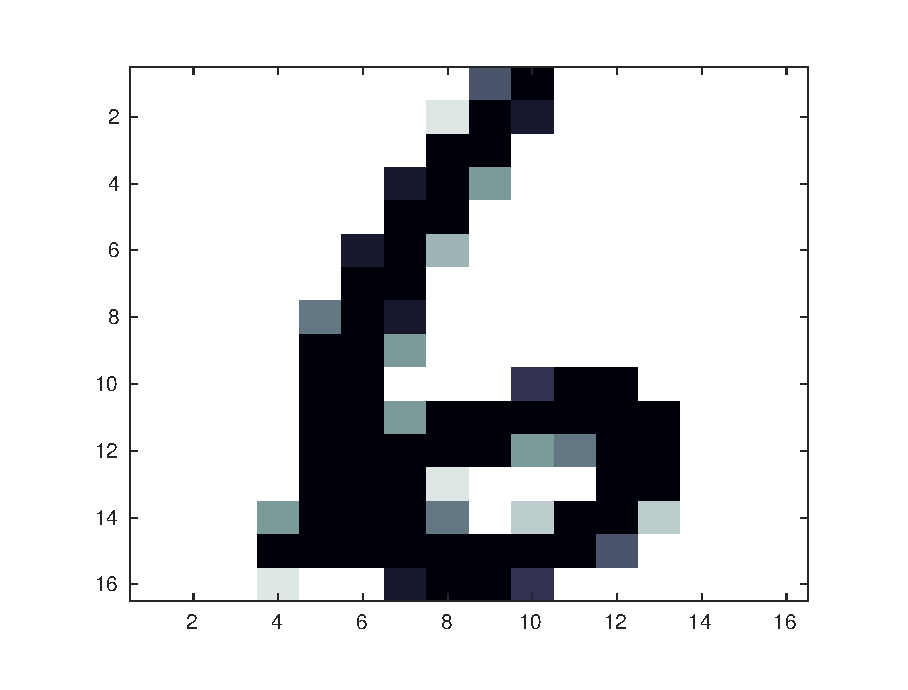
\includegraphics[width = \linewidth]{images/knn/test6.eps}
        \caption{Test digit \(\vec{x}\).}\label{fig:test6}
    \end{subfigure}
    \begin{subfigure}[b]{.3\textwidth}
        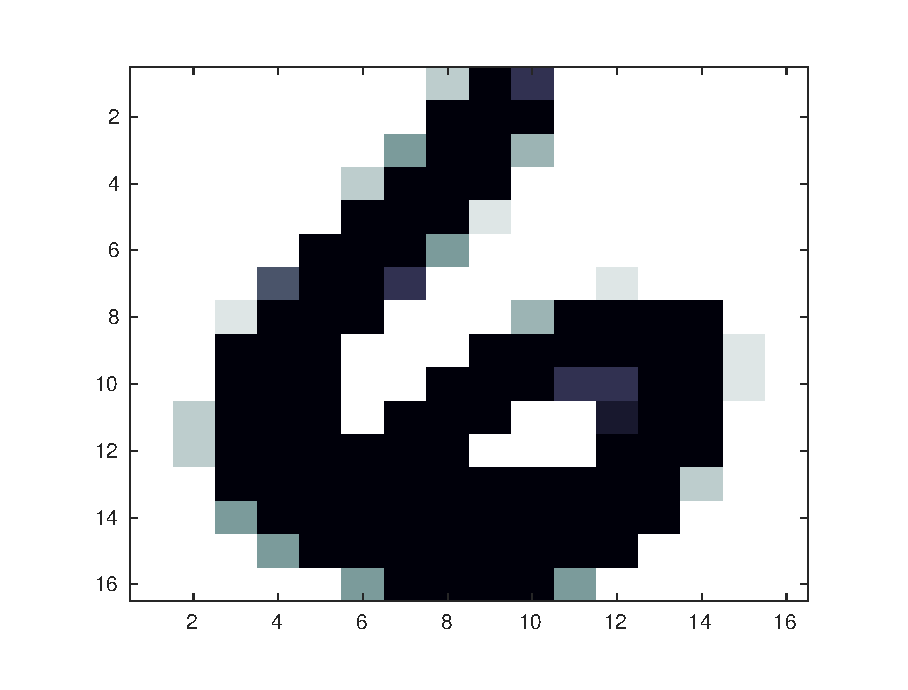
\includegraphics[width = \linewidth]{images/knn/train6.eps}
        \caption{Training data \(\vec{y}\).}\label{fig:train6}
    \end{subfigure}
    \begin{subfigure}[b]{.3\textwidth}
        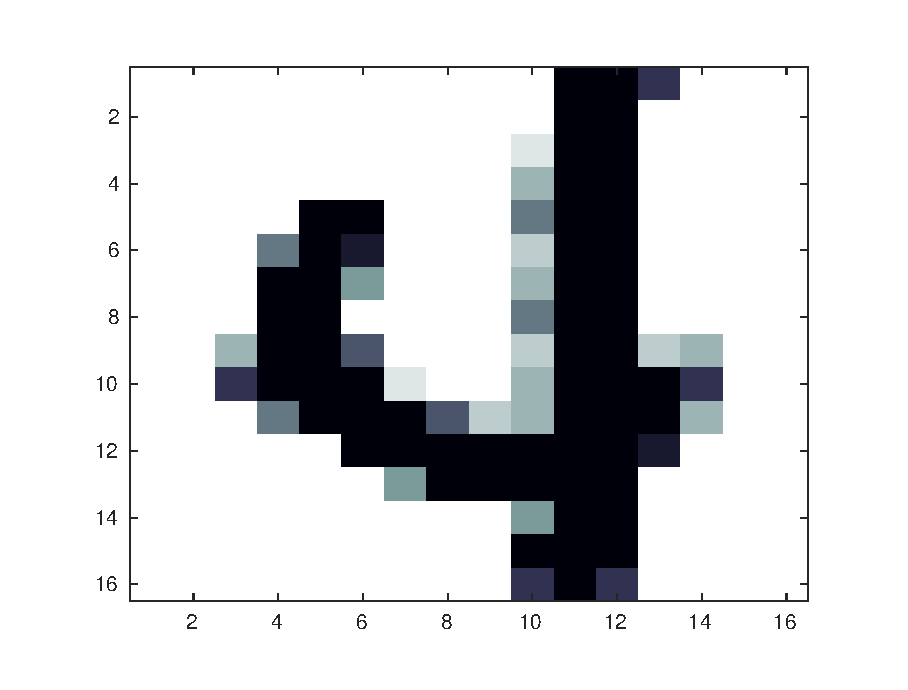
\includegraphics[width = \linewidth]{images/knn/train4.eps}
        \caption{Training data \(\vec{z}\).}\label{fig:train4}
    \end{subfigure}
    \caption{Three different images from the US Postal data set.}
\end{figure}
The first step is to find the distance between \(\vec{x}\) and \(\vec{y}\) and the distance between \(\vec{x}\) and \(\vec{z}\).
In Figures~\ref{fig:difference66}~and~\ref{fig:differenc46} the results of the operations
\[\vec{u} = {(\vec{x} - \vec{y})}^{\circ 2}\text{ and }\vec{v} = {(\vec{x} - \vec{z})}^{\circ 2}\]
can be found.
These operations are the equivalent of taking the pixel wise difference between the two images and then squaring each individual pixel value.
Notice that these operations are present in the definition of the Euclidean distance.
To calculate the distance from this, for both \(\vec{u}\) and \(\vec{v}\) the sum of all the pixel values is taken.
Notice how more overlap between the test and training images lead to ``difference''-vectors with less black values.
\begin{figure}[H]
    \centering
    \begin{minipage}{.3\textwidth}
        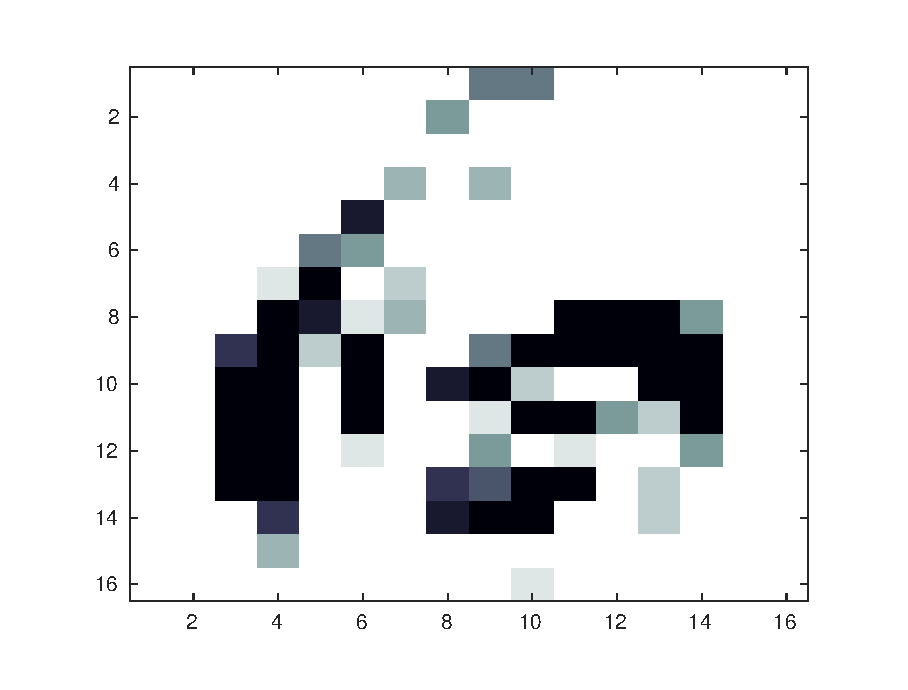
\includegraphics[width = \linewidth]{images/knn/difference66.eps}
        \caption{The vector \(\vec{u}\).}\label{fig:difference66}
    \end{minipage}
    \begin{minipage}{.3\textwidth}
        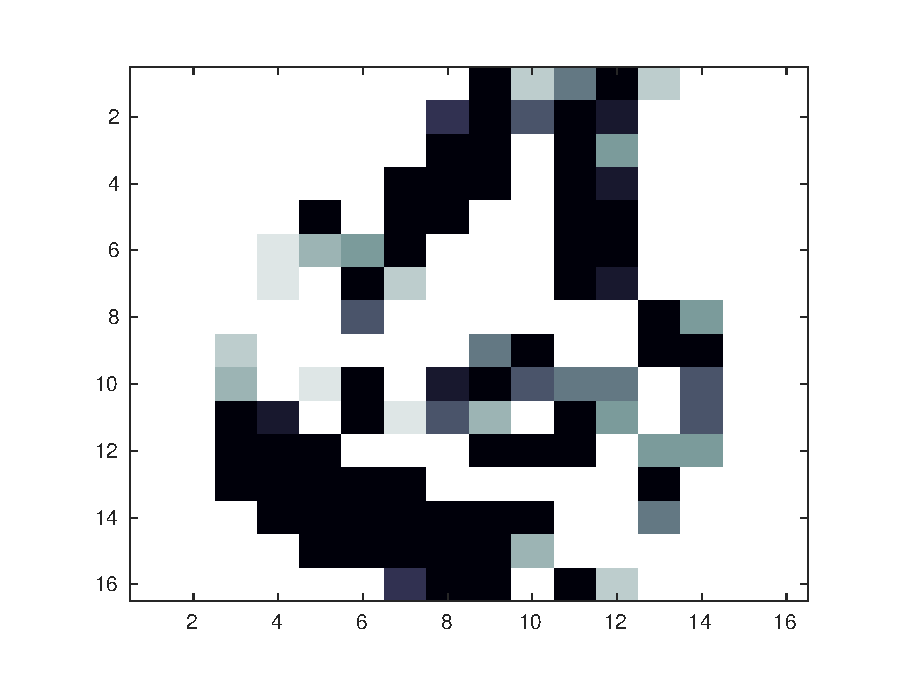
\includegraphics[width = \linewidth]{images/knn/difference46.eps}
        \caption{The vector \(\vec{v}\).}\label{fig:differenc46}
    \end{minipage}
\end{figure}
The sum of all pixel values of \(\vec{u}\) and \(\vec{v}\) are \(12.55\) and \(15.83\).
This means the following:
\begin{align*}
    12.55                                              & < 15.83                                     \\
    \implies \sum_{i = 1}^{256} u_i                    & < \sum_{i = 1}^{256} v_i                    \\
    \implies \sum_{i = 1}^{256} {(x_i - y_i)}^2        & < \sum_{i = 1}^{256} {(x_i - z_i)}^2        \\
    \implies \sqrt{\sum_{i = 1}^{256} {(x_i - y_i)}^2} & < \sqrt{\sum_{i = 1}^{256} {(x_i - z_i)}^2} \\
    \implies \norm{\vec{x} - \vec{y}}                  & < \norm{\vec{x} - \vec{z}}                  \\
    \implies d(\vec{x}, \vec{y})                       & < d(\vec{x}, \vec{z})
\end{align*}
In other words, the result that \(12.55 < 15.83\) implies that \(\vec{x}\) more closely resembles \(\vec{y}\) than \(\vec{z}\).
Since there are only two training samples this also means that the test digit will now be classified as the digit of the most similar image, which is a six.
This is how a digit is classified using the nearest neighbour algorithm in conjunction with the Euclidean distance.

One may note that even though the example was set up to do a correct classification, the difference between \(\vec{u}\) and \(\vec{v}\) is pretty small.
This is related to the fact that the 6 in Figure~\ref{fig:train6} is ``wider'' and ``fatter''.
Furthermore, the Euclidean distance is also susceptible to rotations, scaling and transformations.
The latter of which is illustrated in Figures~\ref{fig:left6}~and~\ref{fig:differenc6left6}.
\begin{figure}[H]
    \centering
    \begin{minipage}{.45\textwidth}
        \centering
        \includegraphics[width = 0.8\linewidth]{images/knn/left6.png}
        \caption{Transposition of \(\vec{x}\).}\label{fig:left6}
    \end{minipage}
    \begin{minipage}{.45\textwidth}
        \centering
        \includegraphics[width = 0.8\linewidth]{images/knn/difference6left6.png}
        \caption{Difference \(\vec{x}\) and its transposition.}\label{fig:differenc6left6}
    \end{minipage}
\end{figure}
The difference between the sum of the elements of Figure~\ref{fig:test6} and the same image shifted left by four pixels is \(17.52\).
This distance is greater than both the other digits.
To deal with these weaknesses the Tangent distance was developed.

\subsubsection{Tangent distance}
As mentioned before, the 1-norm and Euclidean metric are very susceptible to translations and rotations.
The Tangent distance is developed to be invariant with respect to translation, rotation, scaling, shearing, line thickness, and two hyperbolic transforms~\cite{LiweiWang2005}. An example of shearing is the mapping from \((x, y)\) to \((x+2y, y)\).

As we have already established, an image is a point in the 256-dimensional space \(\mathbb{R}^{256}\).
Take a point from this pixel space.
Now, define a transformation.
As example, we take a rotation, such that the parameter corresponds to the angle of the rotation.
Transforming the point according to this rotation yields another point in the pixel space for each angle of rotation.
All points obtained from rotating one point together form a 1-dimensional manifold~\cite{Simard1992, Simard2000}.
It helps to think of this as a line through the pixel space with all slightly rotated versions of the point.
If we take \(P\) to be an image representing a three, then these rotations are the true rotations of \(P\) as can be seen in Figure~\ref{fig:manifold_showcase}.

In case multiple transformations are of interest, the set of transformations can be parametrised by \(n\) parameters. This in turn yields an \(n\)-dimensional manifold.
\begin{figure}[H]
    \centering
    \includegraphics[width = .5\textwidth]{images/knn/manifold_showcase.png}
    \caption{Visual representation of a manifold. Image from Simard et al~\cite{Simard1992}.}\label{fig:manifold_showcase} % background is visible
\end{figure}

The distance between two points can now be defined as the minimum distance between their respective manifolds.
A big problem with this is that the manifold will not be linear, which means that the computation of this distance is a hard non-linear optimization problem~\cite{Keysers2002}.
Alternatively, the distance to the linear approximation of the manifold can be calculated as the approximation is very good for reasonably small angles~\cite{Simard2000}.
The difference can be seen in Figure~\ref{fig:manifold_showcase}, where the resulting rotations of the linear approximation along with tangent vector are shown.
Figure~\ref{fig:manifold_tangent} also shows the difference between the true rotations and the ones created by the linear approximation along with a sketch of the approximation in the pixel space.
Figure~\ref{fig:manifold_distance} visually shows the different distances and how they relate to each other.

\begin{figure}[H]
    \centering
    \begin{minipage}{.45\textwidth}
        \includegraphics[width = \linewidth]{images/knn/manifold_tangent.png}
        \caption{Tangent of manifold~\cite{Simard2000}.}\label{fig:manifold_tangent}
    \end{minipage}\hspace{1em}
    \begin{minipage}{.45\textwidth}
        \includegraphics[width = \linewidth]{images/knn/manifold_distance.png}
        \caption{Distances where \(\vec{P}\) and \(\vec{E}\) are points in the pixel space~\cite{Simard2000}.}\label{fig:manifold_distance}
    \end{minipage}
\end{figure}

The main advantage of this approach using the Tangent distance is accuracy as seven chosen transformations mentioned earlier, which should not influence distance, have less impact on the distance compared to Euclidean distance~\cite{LiweiWang2005}.
Naturally, computing the linear approximation results in a lot of computational overhead, increasing the time complexity.
The results which confirm these statements can be found in Table~\ref{tab:knn_all}.

\begin{table}[H]
    \centering
    \caption{Results of nearest neighbour with \(k = 1\).}\label{tab:knn_all}
    \begin{tabular}{l c c c}
        \toprule
        \textbf{Distance} & 1-norm & Euclidean & Tangent \\
        \textbf{Accuracy} & 0.91   & 0.92      & \00.94  \\
        \textbf{Time (s)} & 7.20   & 6.73      & 59.92   \\ \bottomrule
    \end{tabular}
\end{table}
The code to calculate the tangent distance between two images is taken from Keysers et al~\cite{Keysers2002} and was slightly modified to fit the images with a different dimension.

\subsection{Complexity}\label{s:knn:complexity}
Certain applications of digit recognition require a faster classification time than others, such as self-driving cars as compared to writing input on a tablet.
The time complexity describes the amount of time an algorithm takes to run.
All previous subsections discuss the classification of a single digit.
For this single image a distance needs be calculated to every single training image.
This cannot be avoided, however when a second image needs to be classified the distance to each training image should not have to be calculated all over again as the point distribution stays the same.
Certain data structures, such as the \(k\)-d tree, could reduce the amount of distances that need to be calculated.

Besides the computational cost, \(k\)-nearest neighbour as implemented until now is very sensitive to the composition of the training data.
For example, having a lot of sixes compared to zeros will mean that the number six is much more likely to be chosen for a classification.
To solve this, a lot of variations of kNN such as the weighted \(k\)-nearest neighbour, and \(k\)-d tree nearest neighbour have been developed~\cite{Bhatia2010}.

The computational complexity will be derived where useful.

\subsubsection{Linear Search}
The way the classification problem is solved up until this point is with the use of linear search, sometimes called exhaustive or naive search.
It is the ``normal'' implementation of kNN and does not rely on any structuring of the data.
For each image \(\vec{y}\), the distance between \(\vec{y}\) and every other image in the training set is calculated.
The training images are then sorted on their distance to the image \(\vec{y}\).
The most occurring digit in the top \(k\) is picked as the result of the classification.

A tie happens when the two images closest images have different labels.
The case \(k = 2\) results in 293 ties in the used data set, which is \(14.6\% \) of all cases.
The case \(k = 3\) results in no ties happening, which has to do with the fact that a three-way tie is only possible when the three nearest neighbour all represent a different number.
In case of a tie there are several tie-breaking actions that could be chosen:
\begin{itemize}
    \item Choose a different arbitrary \(k\) until there is no longer a tie~\cite{Pylypiw2017}.
    \item Randomly choose between tied values.
          This is the simplest way, however since there is no reason to make a particular a choice. This typically leads to the lowest accuracy~\cite{Pylypiw2017}.
    \item Start with \(k=2\) and increase \(k\) until the tie is broken~\cite{Pylypiw2017}.
    \item Adding weights to the \(k\) values.
          There are several different functions for assigning weights~\cite{Macleod1987}.
          A simple example is \(\frac{1}{d(\vec{x}, \vec{y})}\) as the vector \(\vec{y}\) has the smallest distance to \(\vec{x}\) of the \(k\)-nearest and therefore has the most influence~\cite{Majewski2012}.
          This solution corresponds to the weighted \(k\)-nearest neighbour mentioned earlier~\cite{Bhatia2010}.
\end{itemize}

Now, we reason about the time complexity for linear search.
Let \(t_r\) be the number of training images and \(t_e\) the number of test images.
Since both test and training images have a fixed dimension of \(16 \times 16\), the time complexity of calculating a distance between two images is \(\mathcal{O}(1)\), which is constant.
To classify one image, \(t_r\) number of distances need to be calculated, so the time complexity is \(\mathcal{O}(t_r)\).
To classify \(t_e\) images, the classification of one image is repeated \(t_e\) times, so the total time complexity is \(\mathcal{O}(t_r \cdot t_e)\).

\subsubsection{\textit{k}-d tree}
Calculating the distance between all training images and test images requires a lot of computation, which in turn takes time.
Recall that training images can also be represented by a vector in the Euclidean space and Euclidean space is a vector space in which all points can be ordered with respect to a single dimension.
The idea is to use these properties to create a data structure, such that a lot of candidates can be pruned.
One such data structure is the \(k\)-dimensional tree, or \(k\)-d tree~\cite{Bentley2002}.

The recursive creation of such a \(k\)-d tree with dimensionality \(2\) will be explained.
All entries in the training data set form a set \(S_0\). Sort all the points with respect to their first dimension, here \(x\) coordinates. Now, take the median point as the root node, in the case of Figure~\ref{fig:tree} this is \(A(50, 50)\). Divide all points into two groups, \(S_1\) and \(S_2\), which contain the points with smaller \(x\) coordinates and larger \(x\) coordinates respectively. Now, do this recursively on \(S_1\) and \(S_2\) while using the next dimension, here \(y\) coordinates. Repeat this while cycling through the dimensions until all points are in the \(k\)-d tree.
A \(k\)-d tree can be built in \(\mathcal{O}(kn \log n)\) time~\cite{Brown2015kdtree}.
According to~\cite{Bentley2002}, the asymptotic running time for nearest neighbour queries is empirically observed to be \(\mathcal{O}(\log n)\).

An example of a query is as follows.
Suppose we want to find the nearest point to the point \textbf{Z}\((60, 85)\).
The first coordinate of \textbf{Z} is bigger than \textbf{A}, so in the tree we traverse to the right side.
The second coordinate of \textbf{Z} is bigger than \textbf{C}, so in the tree we traverse to the right side.
The first coordinate of \textbf{Z} is smaller than \textbf{F}, so in the tree we reach a leaf node and \textbf{F} is thus the closest node.
Now, we draw a circle with radius \(d(\textbf{Z}, \textbf{F}) = 10\).
This circle crosses no splitting boundaries, so there cannot be a point closer than \textbf{F}.
In case the circle does cross a splitting boundary, there can be a closer point, so you have to traverse up the tree a check each element in the branch corresponding to the plane the circle crosses.
\begin{figure}[H]
    \centering
    \includegraphics[width = 0.5\textwidth]{images/plane}\includegraphics[width = 0.5\textwidth]{images/tree}
    \caption{Points in 2-dimensional space (left) stored as nodes in a 2-d tree (right).}\label{fig:tree}
\end{figure}

\subsubsection{Performance}
The asymptotic running time for nearest neighbour queries of \(\mathcal{O}(\log n)\) only holds for relatively small \(k\), where the logarithmic behaviour is observed on a large number of training samples.
Due to the sparsity of the data, for large \(k\) this effect becomes even more pronounced.
For example, for \(k = 16\) a search of a \(k\)-dimensional tree of 76,000 records examines almost every record, which means that (almost) no pruning is happening and that the tree has lost its purpose~\cite{Sproull1991}.
To put this into perspective, the data set in this paper has a dimensionality of \(k = 256\) with only 1,707 training images.
As a result, using the \(k\)-d tree still requires that the distance to all training images needs to be calculated to find the most similar one, while incurring the overhead of precomputing the data structure.
This can be seen in the results in Table~\ref{tab:knn_anthon}.
Since the \(k\)-d tree nearest neighbours queries take as much time as the linear search, the estimated data structure overhead is as much as \(25\% \).
\begin{table}[H]
    \centering
    \caption{Results of kNN on training data set. The time includes preprocessing and the querying of all test images.}\label{tab:knn_anthon}
    \begin{tabular}{l c c c c c}
        \toprule
        \textbf{\(k\)}             & 1    & 2    & 3    & 4    & 5    \\
        \textbf{Accuracy}          & 0.92 & 0.90 & 0.91 & 0.90 & 0.90 \\
        \textbf{Time Linear (s)}   & 0.34 & 0.30 & 0.31 & 0.29 & 0.30 \\
        \textbf{Time k-d tree (s)} & 0.59 & 0.36 & 0.34 & 0.36 & 0.37 \\ \bottomrule
    \end{tabular}
\end{table}
Furthermore, unexpectedly the accuracy only decreases as \(k\) increases.
This can be explained as a combination of sparse data and no labelling errors in the training set.
A consequence of the sparsity of the data is that images with a bigger distance to the unknown image are included and exercise influence on the classification of that image. Paraphrased, this means that more and more irrelevant images are used to classify an image, hence leading to less accurate results.

Note that the times are not comparable with Table~\ref{tab:knn_all}.
This is related to the fact that the algorithm was run on an implementation which is specifically crafted to only be influenced by the time the distance calculation takes without any other optimizations such as to have a level playing field.

\subsection{Approximate methods}\label{s:knn:approximate}
Storing the data in \(k\)-d trees did not prove successful in bringing down the running time for applications with a time constraint.
For these kinds of applications, derivatives of the \(k\)-nearest neighbour method have been developed under the name approximate nearest neighbour.

This class of nearest neighbour techniques exploits redundancy to reduce the computational cost.
The training data set in this paper has 1,707 entries, which contains 252 images representing the number one.
There is guaranteed to be a lot of overlap between these images.
The name contains ``approximate'', because reducing overlap almost always comes in some form of data simplification where some information will be lost.

The term approximate nearest neighbours is a hypernym, meaning that there are many algorithms falling under the name such as locality sensitive hashing, clustering, etcetera~\cite{Rajaraman2011, Bhatia2010}.
Ultimately, approximate nearest neighbour only yields improvement in time complexity and memory use, while sacrificing some accuracy.

\subsubsection{Nearest Mean}
One way to reduce redundancy and overlap is by grouping together duplicate images. All metrics have the properties and results for vectors such that \(\vec{x} = \vec{y}\):
\begin{align*}
    \vec{x}                      & = \vec{y} \implies d(\vec{x}, \vec{y}) = 0                           & \text{See~\cite{Simard1992,Bramwell2007}} \\
    d(\vec{x}, \vec{z})          & \leq d(\vec{x}, \vec{y}) + d(\vec{y}, \vec{z}) = d(\vec{y}, \vec{z})                                             \\
    d(\vec{y}, \vec{z})          & \leq d(\vec{y}, \vec{x}) + d(\vec{x}, \vec{z}) = d(\vec{x}, \vec{z})                                             \\
    \implies d(\vec{x}, \vec{z}) & = d(\vec{y}, \vec{z})
\end{align*}
This proves that the distance from an arbitrary image to two identical training images will be the same.
This means that duplicates in the training data set can be removed without affecting the accuracy of the algorithm.

The sparsity of the data implies that the amount of duplicates in the training set will be very limited, hence this will barely improve the speed.
If more performance is still desired, images with very small differences can then be merged.
The threshold for clustering two images has to be experimented with to find the optimal value.
However, this is a trade-off, since a lower threshold will yield better accuracy, yet a lower performance and vice versa.
Setting the threshold to 0 will give the same results as the ``standard'' nearest neighbours, while setting no bound for the threshold will result in merging everything and yield the nearest mean.

With no bound, all images of the same class are merged into a vector.
This vector will simply be the average image for each class.
On the left side in Figure~\ref{fig:train_3} a normal 3 can be seen beside the ``average'' 3.
Here, the loss of information is also clearly illustrated.
\begin{figure}[H]
    \centering
    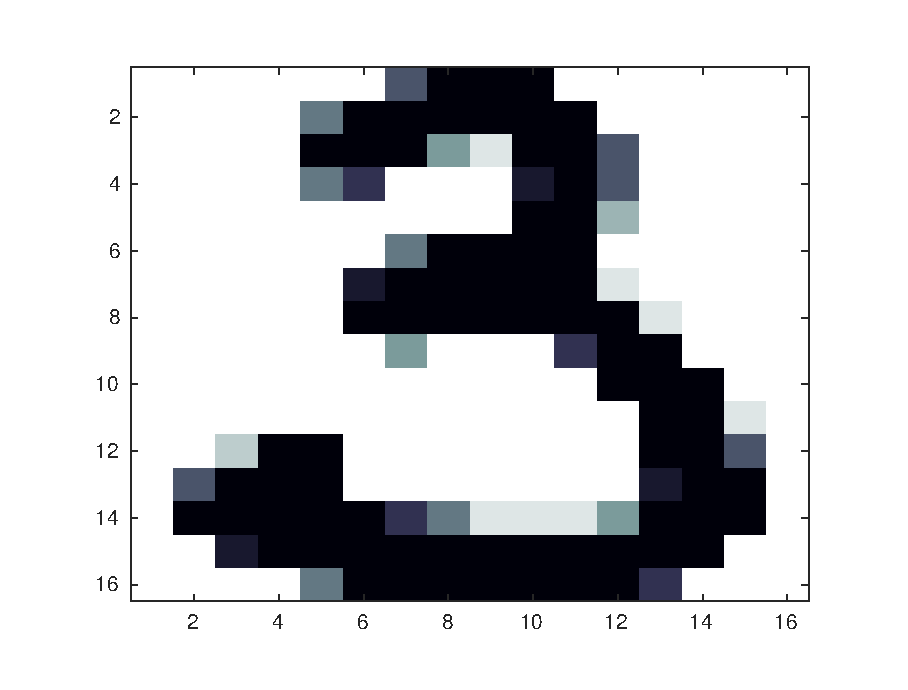
\includegraphics[width = 0.3 \textwidth]{images/train_3.eps}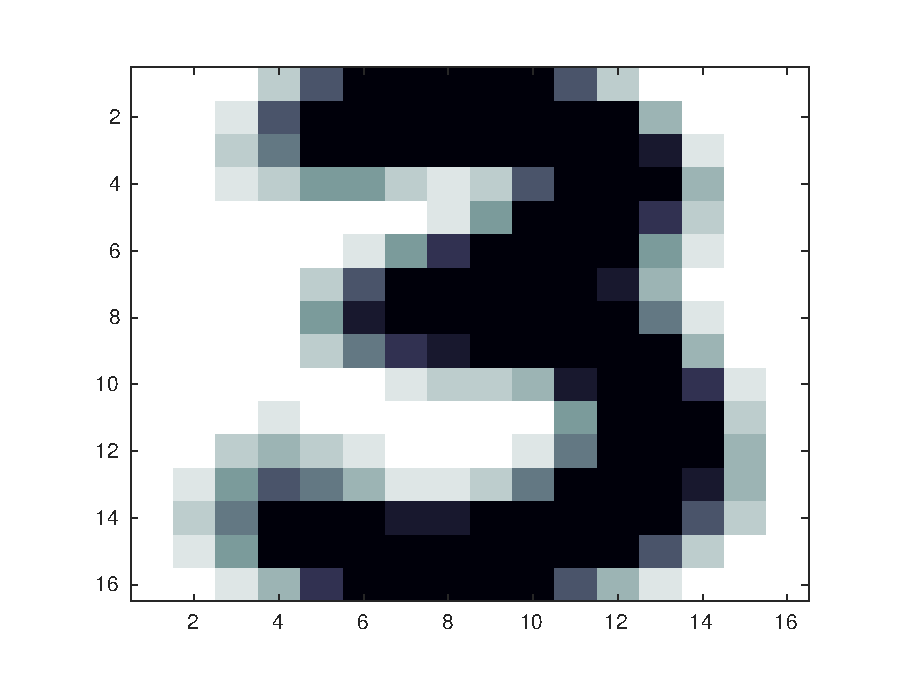
\includegraphics[width = 0.3 \textwidth]{images/average_3.eps}
    \caption{A 3 occurring in the training set and the average 3 vector.}\label{fig:train_3}
\end{figure}
As stated before, the computation of all of the mean images takes \(\mathcal{O}(t_r)\) time, with \(t_r\) the number of training images.
The main advantage of this approach is speed, since each test image has to be checked against only 10 other images.
As a result, a single classification has a time complexity of \(\mathcal{O}(1)\) for an image of a fixed size.
For \(t_e\) number of classifications the total asymptotic computational complexity is \(\mathcal{O}(t_e + t_r)\).

The results, as seen in Table~\ref{tab:mean_anthon}, portray a significant speed advantage over the results seen in Table~\ref{tab:knn_all}.
An important thing to note is that each class now only has one representative.
As a result, the linear approximations of the manifolds cannot overlap with images already present in the training set.
This in turn leads to the Tangent distance yielding a much bigger improvement over the Euclidean distance, while having relatively the same performance penalty.

\begin{table}[H]
    \centering
    \caption{Results of Nearest Mean.}\label{tab:mean_anthon}
    \begin{tabular}{l c c c}
        \toprule
        \textbf{Distance} & 1-norm & Euclidean & Tangent \\
        \textbf{Accuracy} & 0.71   & 0.81      & 0.88    \\
        \textbf{Time (s)} & 0.04   & 0.03      & 0.34    \\
        \bottomrule
    \end{tabular}
\end{table}
Note that the Tangent distance in these tests is implemented in C compiled with Mex, so the time values of the Tangent distance can only be meaningfully compared with the same implementations in this paper.

In this section the distance from a new image to (a subset of) all images in the training set was used to identify images.
The images associated with the same number span a subspace of \(\mathbb{R}^{256}\).
In the next section the distance to this subspace will be used to classify digits instead.
\section{Singular Value Decomposition (SVD)}\label{s:svd_all}
The approach using SVD is similar to, and could even be viewed as an implementation of, the approximate nearest neighbour approach.
The application of kNN to the task of classifying images is known to suffer from various phenomena that arise when analysing high-dimensional spaces.
Problems that we have seen until now that result from this are the severely reduced effectiveness of the \(k\)-d tree and the fact that increasing \(k\) reduces accuracy.
These various phenomena are known as the curse of dimensionality~\cite{Beyer1999}.

Dimensionality reduction is the process of reducing the number of random variables under consideration~\cite{Roweis2000}.
To retain as much information as possible, the data is transformed from the high-dimensional space to a space of fewer dimensions, in a process known as feature extraction.
In this paper, the singular value decomposition~(SVD) is used. This technique is also known as the principal component analysis~(PCA) in the field of statistics.

SVD is regularly researched in the context classifying images of faces and handwritten digits~\cite{Cao2006, Savas2007}.
In this section the SVD and particularly the left-singular vectors are used to classify handwritten digits.

\subsection{Training}\label{s:svd:training}
In this subsection, several concepts of subspaces and the SVD are explained together with their role in the context of image classification.
As mentioned before, it is easier to work with images in the form of a vector as compared to a matrix or grid and therefore, images are flattened first.
Next, a matrix \(\vec{A}_n\) is created for each of the digits, such that the columns consist of all column vectors representing the number \(n\).
Suppose \(a_i\) with \(i = 1, 2, 3, \ldots, k\) are the training vectors representing the number \(n\).
The matrix has the following structure:
\[
    \vec{A}_n =
    \left(
    \begin{array}{cccc}
            \vertbar & \vertbar &        & \vertbar \\
            a_1      & a_2      & \cdots & a_k      \\
            \vertbar & \vertbar &        & \vertbar \\
        \end{array}
    \right).
\]
For example, the columns of the matrix \(\vec{A}_3\) consists of all vectors which are labelled as the number three.

The column space of a matrix \(\vec{A}\) is a space containing all linear combinations of its column vectors.
The column space of \(\vec{A}\) is also called the image or range, \(\mathcal{R}(\vec{A})\), of \(\vec{A}\).
The set of all possible linear combinations is also called the (linear) span or linear hull.

The column space of \(\vec{A}_n\) is now a space containing all linear combinations of the images that represent the number \(n\).
Each number has a subspace of the pixel space associated with it.
This can already be used for classification.
All that needs to be done is to calculate this distance between the test image and all linear subspaces. The number associated with the subspace that is closest to the test image is chosen as the label of the test image.

Each linear subspace is spanned by a lot of vectors.
This results in a very expensive distance computation and a lot of overlap of the different subspaces.
An image that is in both subspaces will have a distance of zero to both, so overlapping subspaces are guaranteed to result in worse accuracy.

This way of classifying is thus both very slow and inaccurate.
To improve this, the SVD will be used to find vectors that span smaller subspaces.

\textbf{Theorem. (SVD)} \textit{Any matrix \(\vec{A}\in \mathbb{R}^{m \times n}\), with \(m\geq n\) can be factorised
    \[\vec{A} = \vec{U}\vec{\Sigma}\vec{V}^T,\]
    where \(\vec{U}\in\mathbb{R}^{m\times m}\) and \(\vec{V}\in\mathbb{R}^{n\times n}\) orthogonal, and \(\vec{\Sigma}\in\mathbb{R}^{m\times n}\) is rectangular diagonal,
    \[\Sigma = \textnormal{diag}(\sigma_1, \sigma_2, \ldots, \sigma_n),\]
    \[\sigma_1\geq\sigma_2\geq\cdots\geq\sigma_n\geq 0.\]
    The values on the diagonal of the matrix \(\vec{\Sigma}\) are known as the singular values, while the columns of \(\vec{U}\) and \(\vec{V}\) are called the left-singular and right-singular vectors respectively~\cite{Elden2011, Savas2007}.}

The derivation below shows that the left-singular vectors are the set of eigenvectors of \(\vec{A}\vec{A}^T\).
These are thus obtained by solving the eigenvalue problem \(\vec{A}\vec{A}^T\vec{x} = \sigma \vec{x}\).
\begin{align*}
    \vec{A}                      & = \vec{U}\vec{\Sigma}\vec{V}^T                                 \\
    \vec{A}^T                    & = \vec{V}\vec{\Sigma}^T\vec{U}^T                               \\
    \Rightarrow \vec{A}\vec{A}^T & = \vec{U}\vec{\Sigma}\vec{V}^T\vec{V}\vec{\Sigma}^T\vec{U}^T   \\
    \Rightarrow \vec{A}\vec{A}^T & = \vec{U}\vec{\Sigma}(\vec{V}^T\vec{V})\vec{\Sigma}^T\vec{U}^T \\
    \Rightarrow \vec{A}\vec{A}^T & = \vec{U}(\vec{\Sigma}\vec{\Sigma}^T)\vec{U}^T
\end{align*}
\(\vec{\Sigma}\vec{\Sigma}^T\) is a real symmetric matrix, so the eigenvectors can be chosen to be orthogonal.
The remainder of this section assumes that the eigenvectors are orthonormal, which is obtained by dividing the eigenvectors by their norm.

We define \(p\) as the rank of \(\vec{A}\), then we have the following:
\begin{align*}
    \mathcal{R}(\vec{A}) & = \{\vec{A}\vec{x}:\vec{x}\in\mathbb{R}^n\}                      \\
                         & = \{\vec{U}\vec{\Sigma}\vec{V}^T\vec{x}:\vec{x}\in\mathbb{R}^n\} \\
                         & = \{\vec{U}\vec{\Sigma}\vec{y}:\vec{y}\in\mathbb{R}^n\}          \\
                         & = \{\sum_{j = 1}^n \vec{u}_j c_j:c_j\in\mathbb{R}\}            \\
                         & = \mathcal{R}(\left(\begin{array}{cccc}
            \vertbar & \vertbar &        & \vertbar \\
            u_1      & u_2      & \cdots & u_p      \\
            \vertbar & \vertbar &        & \vertbar \\
        \end{array}\right)).
\end{align*}
This means that the first \(n\) columns of \(\vec{U}\) form an orthonormal basis for \(\mathcal{R}(\vec{A})\), that is the first \(k\) columns of \(\vec{U}\) are orthogonal and they are all unit vectors~\cite{Cao2006}.
In Section~\ref{s:svd} the importance of orthonormality will be explained.
To clarify, the first \(k\) columns of \(\vec{U}_n\) form the orthonormal basis, so from this point onwards \(\vec{U}_n\) refers to the first \(p\) columns of \(\vec{U}_n\).

The fact that the singular values are in decreasing order means that the corresponding left-singular vectors are in decreasing order of importance.
Intuitively, the first \(k\) columns of \(\vec{U}\) span a space using the \(k\) most important orthogonal directions.
The first three columns of \(\vec{U}_3\) are visible in Figures~\ref{fig:svd_u1},~\ref{fig:svd_u2}~and~\ref{fig:svd_u3}.

\begin{figure}[H]
    \centering
    \begin{minipage}{0.3\textwidth}
        \includegraphics[width = \textwidth]{images/svd/U1.png}
        \caption{Column 1 of \(\vec{U}_3\).}\label{fig:svd_u1}
    \end{minipage}
    \begin{minipage}{0.3\textwidth}
        \includegraphics[width = \textwidth]{images/svd/U2.png}
        \caption{Column 2 of \(\vec{U}_3\).}\label{fig:svd_u2}
    \end{minipage}
    \begin{minipage}{0.3\textwidth}
        \includegraphics[width = \textwidth]{images/svd/U3.png}
        \caption{Column 3 of \(\vec{U}_3\).}\label{fig:svd_u3}
    \end{minipage}
\end{figure}

In this section several concepts were explained and how they are useful in the context of image classification.
In the next subsection these concepts, and the SVD in particular, together with some mathematical operations will be used to identify the images from the test set.

\subsection{Classification}
In this section the classification procedure using these ideas is explained in more detail and more information is given with regard to finding the distance to a linear subspace.

\subsubsection{Subspace spanned by training vectors}
The distance between an image and a subspace cannot be computed directly.
To do this, the distance between an image and its orthogonal projection on the subspace needs to be calculated instead.

\begin{figure}[H]
    \centering
    \includegraphics[width = 0.6\textwidth]{images/svd/orth_proj.png}
    \caption{Orthogonal projection on the column space of \(\vec{A}\), or col\((\vec{A})\)~\cite{Erichson2016}.}\label{fig:orth_proj}
\end{figure}

Suppose that \(\vec{x}\) is the vector that needs to be classified and that \(\hat{\vec{x}} = \vec{P}_n\vec{x}\) is the orthogonal projection of \(\vec{x}\) on the subspace representing the number \(n\).
The distance between \(\vec{x}\) and \(\hat{\vec{x}}\) is (see Figure~\ref{fig:orth_proj})
\[\norm{\vec{x} - P\vec{x}} = \big\lVert\vec{x} - \vec{A}_n{(\vec{A}_n^T \vec{A}_n)}^{-1}\vec{A}_n^T\vec{x}\big\rVert_2. \]

For each new vector the distance to each subspace is calculated.
Suppose that the closest subspace is \(\mathcal{R}(\vec{A}_n)\), which would mean that \(\vec{x}\) is classified as the number \(n\).
Notice that the column space of \(\vec{A}_n\) must be spanned by linearly independent vectors for the inverse of \(\vec{A}_n^T \vec{A}_n\) to exist.

Intuitively, the linear projection of a vector is in fact the best approximation of the vector using a linear combination of the basis vectors.
An image representing the number three (Figure~\ref{fig:svd_test3}) and number nine (Figure~\ref{fig:svd_test9}) can be found below.
To see how this projection affects the image, the orthogonal projections on the column space of \(\vec{A}_3\) of those numbers can be found besides them in Figures~\ref{fig:svd_test3_proj}~and~\ref{fig:svd_test9_proj} respectively.
Note that both Figure~\ref{fig:svd_test3}~and~\ref{fig:svd_test9} are not from the training set, since a projection of a training image representing the number \(n\) on the range of \(\vec{A}_n\) is just the vector itself.

\begin{figure}[H]
    \centering
    \begin{minipage}{0.45\textwidth}
        \includegraphics[width = \textwidth]{images/svd/test3.png}
        \caption{Image representing a 3 from the test set.}\label{fig:svd_test3}
    \end{minipage}
    \hspace{1em}
    \begin{minipage}{0.45\textwidth}
        \includegraphics[width = \textwidth]{images/svd/test3_proj.png}
        \caption{Orthogonal projection of Figure~\ref{fig:svd_test3} on the range of \(\vec{A}_3\).}\label{fig:svd_test3_proj}
    \end{minipage}
\end{figure}
\begin{figure}[H]
    \begin{minipage}{0.45\textwidth}
        \includegraphics[width = \textwidth]{images/svd/test9.png}
        \caption{Image representing a 9 from the test set.}\label{fig:svd_test9}
    \end{minipage}
    \hspace{1em}
    \begin{minipage}{0.45\textwidth}
        \includegraphics[width = \textwidth]{images/svd/test9_proj.png}
        \caption{Orthogonal projection of Figure~\ref{fig:svd_test9} on the range of \(\vec{A}_3\).}\label{fig:svd_test9_proj}
    \end{minipage}
\end{figure}

Recall that the column space of \(\vec{A}_3\) contains all linear combinations of the training images representing a three.
We expect there to be a linear combination closely matching the number three, while no such combination for the number nine exists.
Figures~\ref{fig:svd_test3_proj}~and~\ref{fig:svd_test9_proj} confirm this expectation as the projection of an image representing the number three on \(\mathcal{R}(\vec{A}_3)\) yields a very similar image to the original, while projecting a nine on this space introduces a lot of noise.

\subsubsection{Using the SVD}\label{s:svd}
The first step to classify digits using the SVD is to create the same matrices \(\vec{A}_n\) for each digit \(n\) as created before.
We define \(k_n\) as rank\((\vec{A}_n)\), avoiding having to write rank\((\vec{A}_n)\) everywhere.
As mentioned in Section~\ref{s:svd:training}, the singular value decomposition of each \(\vec{A}_n\) results in the matrix \(\vec{U}_n\), which is a \(256\times k_n\) matrix whose columns span \(\mathcal{R}(\vec{A}_n)\).
Hence, the columns of \(\vec{U}_n\) are \(u_1, \ldots, u_{k_n}\).
So \(\vec{U}_n^T\) and \(\vec{U}_n\) are:
\begin{align*}
    \vec{U}_n^T = \left(
    \begin{array}{ccc}
            \horzbar & u_1^T    & \horzbar \\
            \horzbar & u_2^T    & \horzbar \\
                     & \vdots &          \\
            \horzbar & u_{k_n}^T  & \horzbar
        \end{array}
    \right),
     &  &
    \vec{U}_n = \left(\begin{array}{cccc}
            \vertbar & \vertbar &        & \vertbar \\
            u_1      & u_2      & \cdots & u_{k_n}    \\
            \vertbar & \vertbar &        & \vertbar
        \end{array}
    \right).
\end{align*}
As mentioned before, the column vectors of \(\vec{U}_n\) are all orthogonal and unit vectors.
This means that \(u_i \cdot u_i = 1\) and \(u_i \cdot u_j = 0\) for all \(i \neq j\), where \(\cdot \) denotes the dot product.
The matrix multiplication of \(\vec{U}_n^T\) and \(\vec{U}_n\) then yields:
\begin{align*}
    \vec{U}_n^T \vec{U}_n & = \left(
    \begin{array}{cccc}
            u_1\cdot u_1   & u_1\cdot u_2   & \cdots & u_1\cdot u_{k_n}   \\
            u_2\cdot u_1   & u_2\cdot u_2   & \cdots & u_2\cdot u_{k_n}   \\
            \vdots         &                & \ddots & \vdots           \\
            u_{k_n}\cdot u_1 & u_{k_n}\cdot u_2 & \cdots & u_{k_n}\cdot u_{k_n}
        \end{array}\right) \\
                          &
    = \left(\begin{array}{cccc}
            1      & 0 & \cdots & 0      \\
            0      & 1 & \cdots & 0      \\
            \vdots &   & \ddots & \vdots \\
            0      & 0 & \cdots & 1
        \end{array}
    \right)                           \\
                          & = I
\end{align*}

Substituting this in the formula for the distance between a vector and its orthogonal projection yields:
\begin{align*}
    \norm{\vec{x} - P\vec{x}} & = \big\rVert\vec{x} - \vec{U}_n{(\vec{U}_n^T \vec{U}_n)}^{-1}\vec{U}_n^T\vec{x}\big\rVert \\
                              & = \norm{\vec{x} - \vec{U}_n I^{-1}\vec{U}_n^T\vec{x}}                                     \\
                              & = \norm{\vec{x} - \vec{U}_n\vec{U}_n^T\vec{x}}
\end{align*}
Therefore, the distance between a vector and a subspace spanned by the columns of \(\vec{U}_n\) is\\ \(\norm{\vec{x} - \vec{U}_n\vec{U}_n^T\vec{x}}\).

In Table~\ref{tab:nr_of_basis}, the subspace corresponding to each number is stated with the amount of basis vectors and the amount of column vectors of \(\vec{A}_n\).
Note that the training set for some numbers has an equal amount of basis vectors compared to orthonormal vectors.
This means that every vector in \(\vec{A}_n\) was already linearly independent.
\begin{table}[H]
    \centering
    \caption{Number of basis vectors used to span the different subspaces.}\label{tab:nr_of_basis}
    \begin{tabular}{lcccccccccc}
        \toprule
        \textbf{\textit{n}}                                         & 0   & 1   & 2   & 3   & 4   & 5   & 6   & 7   & 8   & 9   \\
        \textbf{\(k_n\)} & 245 & 100 & 202 & 131 & 122 & 88 & 151 & 166 & 144 & 132 \\
        \textbf{number of columns \(\vec{A}_n\)}       & 319 & 252 & 202 & 131 & 122 & 88  & 151 & 166 & 144 & 132 \\
        \bottomrule
    \end{tabular}
\end{table}
\subsection{Performance}
The difference in speed between using linearly independent columns of \(\vec{A}_n\) and the orthonormal columns of \(\vec{U}_n\) consists of two main parts.
First, the basis columns of \(\vec{A}_n\) must be chosen. To do this, each column vector needs to be checked whether or not they are a linear combination of the previous columns.
This is an expensive computation when compared to computing the SVD.\@
The second part responsible for the difference is the distance function. In Section~\ref{s:svd} we saw that the orthonormality condition resulted in a simplified calculation.
In Table~\ref{tab:svd_all} the difference between the running time of both distances can be seen.

At this point, all the columns of \(\vec{U}_n\) are used to span the space on which the vectors are projected.
As mentioned before, the singular vectors are ordered from important to less important.
The first \(r\) vectors of \(\vec{U}_n\) span a subspace of \(\mathcal{R}(\vec{A})\) that contains the most important features for the number \(n\).
A feature then is a certain combination of pixel values.
The amount of orthogonal vectors \(r\) to be taken as our basis is yet to be determined.

The choice for \(r\) must be independent from the test set, so different amounts of vectors are tested on the training set and their results are plotted in Figure~\ref{fig:r_values_acc}.
A projection onto a subspace spanned by more elements naturally has a higher computational cost.
Figure~\ref{fig:r_values_time} shows a clear upwards trend with respect to the time the algorithm takes.
The slight peak in Figure~\ref{fig:r_values_time} can be explained by caching optimisations between subsequent runs and would disappear when repeating this test multiple times.

\begin{figure}[H]
    \centering
    \begin{minipage}{0.45\textwidth}
        \includegraphics[width = \textwidth]{images/svd/r_values.png}
        \caption{Accuracy plotted against \(r\) values.}\label{fig:r_values_acc}
    \end{minipage}
    \begin{minipage}{0.45\textwidth}
        \includegraphics[width = \textwidth]{images/svd/time.png}
        \caption{Time plotted against \(r\) values.}\label{fig:r_values_time}
    \end{minipage}
\end{figure}

For a better overview, some data values at different intervals can be found in Table~\ref{tab:svd_all}.
The time difference between the simplified distance based on the orthonormality condition and the standard linear independence can also be seen here.
The graph in Figure~\ref{fig:r_values_acc} indicates that \(r = 15\) strikes a good balance between speed and accuracy.

\begin{table}[H]
    \centering
    \caption{Results of SVD classifier.}\label{tab:svd_all}
    \begin{tabular}{lccccccc}
        \toprule
        \textbf{\(r\) value} & 1    & 2    & 5    & 10   & 15   & 20   & 25   \\
        \textbf{Accuracy}    & 0.80 & 0.86 & 0.90 & 0.93 & 0.94 & 0.94 & 0.94 \\
        \textbf{Time orthonormal (s)}    & 0.62 & 0.80 & 0.68 & 0.80 & 0.90 & 1.08 & 1.16 \\
        \textbf{Time linear independent (s)}    & 1.17 & 1.57 & 1.86 & 2.19 & 2.58 & 3.23 & 3.95 \\
        \bottomrule
    \end{tabular}
\end{table}

The last two sections, kNN and SVD, tried to classify digits by computing the distance between a new image and other objects to determine the label.
Another entirely different way of doing this is by constructing a model based on the training images.
In the next section a neural network will be used to label the image.
\section{Neural Network (NN)}\label{s:neural_network}
Another popular way of solving the problem is through the use of Artificial Intelligence~(AI)~\cite{Ciresan2010}. AI is, at the time of writing, a hot topic with Artificial Neural Networks (ANN) receiving special attention.
In this section, a simple feedforward neural net will be created to attempt the classification of the digit from the data set.
The neural net created by Higham will be taken as a basis~\cite{Higham2018}.
The XOR problem based on the logical exclusive-or operator is a test problem that will be solved to showcase the different elements of a neural network~\cite{Shiffman2018}.

In Section~\ref{s:nn:structure} the structure of a neural network is explained.
Section~\ref{s:fp} contains information about forward propagation, followed by the loss function in Section~\ref{s:loss}.
The way a neural network is trained can be found in Section~\ref{s:training}.
The choices for the example problem are motivated in Section~\ref{s:xor}. Section~\ref{s:perf} analyses the results of the neural network that solves the XOR problem.
Finally, the discussed concepts are applied to the classification problem in Section~\ref{s:digit_recognition}.

\subsection{Structure}\label{s:nn:structure}
There are many different complex structures such as recurrent or convolutional neural networks, however for simplicity we will focus on a feedforward neural network.
A feedforward neural network has two main components: nodes, often called neurons, and edges.
A node can have a value which is dependent on the values of nodes connected to it, the weights of the edges, and optionally the bias.
Typically, these artificial neurons are aggregated into layers (see Figure~\ref{fig:neural_net}).

The first layer is called the input layer.
This layer contains the input neurons, which are the neurons with a direct correspondence to the input.
The last layer is called the output layer.
The calculated values in the output neurons are the final result and thus output of the neural network.
All other layers are called hidden layers as their functionality is not exposed to the user.
In the example, illustrated by Figure~\ref{fig:neural_net}, there is only one hidden layer.
\def\layersep{5.3cm}
\begin{figure}[H]
    \centering
    \begin{tikzpicture}[shorten >=1pt,->,draw=black!50, node distance=\layersep]
      \tikzstyle{every pin edge}=[<-,shorten <=1pt]
      \tikzstyle{neuron}=[circle,fill=black!25,minimum size=17pt,inner sep=0pt]
      \tikzstyle{input neuron}=[neuron, fill=green!50];
      \tikzstyle{output neuron}=[neuron, fill=red!50];
      \tikzstyle{hidden neuron}=[neuron, fill=blue!50];
      \tikzstyle{annot} = [text width=4em, text centered]
  
      % Draw the input layer nodes
      \foreach \name / \y in {1,...,2}
      % This is the same as writing \foreach \name / \y in {1/1,2/2,3/3,4/4}
          \node[input neuron, pin=left:Input \# \y] (I-\name) at (0,4*-\y + 3) {\(x_{\y}\)};
  
      % Draw the hidden layer nodes
      \foreach \name / \y in {3,...,5}
          \path[yshift=1cm]
              node[hidden neuron] (H-\name) at (\layersep,2*-\y + 4) {\(x_{\y}\)};
  
      % Draw the output layer node
      \node[output neuron,pin={[pin edge={->}]right:Output}, right of=H-4] (0) {\(x_6\)};
  
      % Connect every node in the input layer with every node in the
      % hidden layer.
      \foreach \source in {1,...,2}
          \foreach \dest in {3,...,5}
              \path (I-\source) edge (H-\dest);
  
      % Connect every node in the hidden layer with the output layer
      \foreach \source in {3,...,5}
          \path (H-\source) edge (0);
  
      % Annotate the layers
      \node[annot,above of=H-3, node distance=1cm] (hl) {Hidden layer};
      \node[annot,left of=hl] {Input layer};
      \node[annot,right of=hl] {Output layer};
      \draw (I-1) -- (H-3) node[midway, above]{\(w_1\)};
      \draw (I-2) -- (H-3) node[near start, above]{\(w_2\)};
      \draw (I-1) -- (H-4) node[midway, above]{\(w_3\)};
      \draw (I-2) -- (H-4) node[midway, below]{\(w_4\)};
      \draw (I-1) -- (H-5) node[near start, below]{\(w_5\)};
      \draw (I-2) -- (H-5) node[midway, below]{\(w_6\)};
      \draw (H-3) -- (0) node[midway, above]{\(w_7\)};
      \draw (H-4) -- (0) node[midway, above]{\(w_8\)};
      \draw (H-5) -- (0) node[midway, below]{\(w_9\)};
  \end{tikzpicture}


    \caption{Neural network.}\label{fig:neural_net}
\end{figure}
The sizes of the input and output layers are often largely dictated by the problem that you are trying to solve.
Generally, deciding on the number of hidden layers and the number of nodes within each layer is not an exact science.
Rules of thumb have been suggested, however there is no widely accepted technique~\cite{Higham2018}.

One property of a feedforward neural network is that edges can only be connected between two consecutive layers.
Consequently, the value of all nodes in the first layer need to be calculated, then the values in the nodes of the second layer and so on.
The process of calculating the nodes is aptly named forward propagation.

\subsection{Forward propagation}\label{s:fp}
First, forward propagation is illustrated on the XOR example.
Then, a more general formula is derived and some notation is introduced.

The input of a neural network consists of values.
The forward propagation of the example, seen in Figure~\ref{fig:neural_net}, goes as follows:
\begin{align*}
    x_1 & = \text{given by input}, & x_3 & = f(w_1\cdot x_1 + w_2\cdot x_2 + b_3), & x_6 & = f(w_7\cdot x_3 + w_8\cdot x_4+ w_9\cdot x_5 + b_6), \\
    x_2 & = \text{given by input}, & x_4 & = f(w_3\cdot x_1 + w_4\cdot x_2 + b_4),                                                               \\
        &                          & x_5 & = f(w_5\cdot x_1 + w_6\cdot x_2 + b_5),
\end{align*}

Notice that these equations can easily be written in matrix form.
These matrices will be referred to as the weight matrices.
This yields the following:
\begin{align*}
    \begin{pmatrix}
        x_3 \\x_4\\x_5
    \end{pmatrix}
    =
    f\left(
    \begin{pmatrix}
        w_1 & w_2 \\
        w_3 & w_4 \\
        w_5 & w_6
    \end{pmatrix}
    \begin{pmatrix}
        x_1 \\x_2
    \end{pmatrix}
    +
    \begin{pmatrix}
        b_3 \\b_4\\b_5
    \end{pmatrix}
    \right), &  &
        x_6
    =
    f\left(
    \begin{pmatrix}
        w_7 & w_8 & w_9
    \end{pmatrix}
    \begin{pmatrix}
        x_3 \\ x_4\\ x_5
    \end{pmatrix}
    +
        b_6
    \right).
\end{align*}

A simple substitution yields the following expression for computing the output in a single step:
\[
        x_6
    =
    f\left(
    \begin{pmatrix}
            w_7 & w_8 & w_9
        \end{pmatrix}
    f\left(
        \begin{pmatrix}
                w_1 & w_2 \\
                w_3 & w_4 \\
                w_5 & w_6
            \end{pmatrix}
        \begin{pmatrix}
                x_1 \\x_2
            \end{pmatrix}
        +
        \begin{pmatrix}
                b_3 \\b_4\\b_5
            \end{pmatrix}
        \right)
    +
            b_6
    \right).
\]

The function \(f\) is called the activation function.
Popular choices for this function are the linear function \(f(x) = x\), the Rectified linear unit (ReLU) function \(f(x) = x\cdot\mathbbm{1}\{x > 0\} \), and the sigmoid function \(f(x) = \sigma(x) = 1/(1+e^{-x})\)~\cite{Higham2018}.
Furthermore, the XOR problem has outputs that can be divided into two classes, true and false, making it a classification problem.
We will take the sigmoid function as the activation function as it is typically chosen in case of classification problems.

For use further in this paper, a general formula is useful.
A general formula is thus derived and some notation is introduced.
Let \(\ell \) be a number corresponding to a layer, let \(\vec{W}^{[\ell]}\) be the weight matrix of layer from layer \(\ell - 1\) to \(\ell \), and let \(\vec{b}^{[\ell]}\) be the biases of layer~\(\ell \).
We define the weighted input of layer \(2 \leq \ell \leq L \) before and after the activation function to be
\begin{align*}
    \vec{z}^{[\ell]} & = \vec{W}^{[\ell]}\vec{a}^{[\ell - 1]} + \vec{b}^{[\ell]}, \\
    \vec{a}^{[\ell]} & = f\left(\vec{z}^{[\ell]}\right),
\end{align*}
where \(L\) is the number of layers of the neural net and where \(a^{[1]}\) corresponds to the input.

The last, and arguably the most important, thing that is needed is a way to improve the weights and biases such that the network as a whole behaves as desired.
Changing the weights and biases for the purpose of improving performance is called training a neural network.
Before a network can be trained, a loss function needs to be computed.

\subsection{Loss function}\label{s:loss}
The loss function, also known as the cost function, is necessary to gauge the performance of the neural network.
A loss function takes the predicted output, \(x_p\in \{0, 1, \ldots, 9\} \), and the actual output, \(x_6\) as inputs and gives a measure of difference between the two.
In this paper the Mean Squared Error (MSE) is used, where \(n\) is the number of training samples.
The MSE is differentiable and has some other convenient properties, which made it very popular for feedforward neural networks such as this one.
The formula is displayed below.
\[C = \frac{1}{n}\sum_{i = 1}^n {(x_6 - x_p)}^2.\]

\subsection{Training the network}\label{s:training}
Training the network is the act of improving the weights and biases in such a way that the neural network behaves as desired.
The two ways discussed in this paper of improving these are through neuroevolution and back propagation.
Before the weights can be improved, initial weights need to be chosen.
There are several ways to pick these, however in this paper for the sake of simplicity they are initialised to a random number.
This can be any random number, however since very big or small values make the process slower we take random numbers from a normal distribution.

\subsubsection{Neuroevolution}
Neuroevolution (NE) is the artificial evolution of neural networks using Genetic Algorithms (GA).
GA are inspired by the process of natural selection.
Neuroevolution starts with creating several neural networks initialised with random weights and biases.
Then the models are tested on the training set and given a fitness score based on how well they performed.
The fittest neural networks have a chance to create so-called offspring, which is a new neural network with a combination of the parents weights and biases.
For each of the fittest there is also a chance to mutate, which randomly changes the weights by some small amount~\cite{Whitley1993}.

There are also more advanced NE algorithms such as the Neuroevolution with Augmenting Topology (NEAT).
Mutations with NEAT also include the possibility to change the topology or structure of the network~\cite{Stanley2002}.

\subsubsection{Gradient descent}
A popular way of improving an NN is through gradient descent with back propagation.
In Section~\ref{s:loss}, the loss function has been defined, which consists only out of the weights and inputs \(x_1, x_2\), and \(x_3\).
That makes this an optimisation problem, where the loss function needs to be minimised.
The calculation of the gradient requires the loss function to be differentiable and hence also continuous.
Even though there are solutions to solve this, however in this case this would add unnecessary complexity.
Differentiable activation functions are thus easier to work with and hence are generally preferred.

To make use of back propagation, first define the error in the \(j\)th neuron to be
\begin{align*}
    \delta^{[\ell]}_j = \frac{\partial C}{\partial z^{[\ell]}_j}, &  & \text{for } 2\leq j\leq n \text{ and }1 \leq j \leq n_\ell
\end{align*}
where \(n_\ell \) is the number of neurons in layer \(\ell \).
We point out that the usage of the term error is somewhat ambiguous.
The idea of referring to \(\delta^{[\ell]}_j\) as an error seems to have arisen because the cost function can only be minimum if all partial derivatives are zero, so \(\delta^{[\ell]}_j = 0\) is a useful goal.

Substituting the various formulas together with the chain rule, which can be found in the paper of Higham et al~\cite{Higham2018}, yields the following:\\
\textbf{Lemma~\cite{Higham2018}. }\textit{We have
    \begin{align}
        \vec{\delta}^{[L]}
         & = \sigma'(\vec{z}^{[L]})\circ (\vec{a}^L - \vec{x}_1),                                 \\
        \vec{\delta}^{[\ell]}
         & = \sigma'(\vec{z}^{[\ell]})\circ {(\vec{W}^{[\ell + 1]})}^T \vec{\delta}^{[\ell + 1]},
         & \textnormal{for }2\leq \ell \leq L -1,                                                 \\
        \frac{\partial C}{\partial w^{[\ell]}_{jk}}
         & = \delta^{[\ell]}_j a^{[\ell - 1]}_k,
         & \textnormal{for }2\leq \ell \leq L,\label{l:cw}                                        \\
        \frac{\partial C}{\partial b^{[\ell]}_j}
         & = \delta^{[\ell]}_j,
         & \textnormal{for }2\leq \ell \leq L.\label{l:cb}
    \end{align}}

Here, \(\circ \) also denotes the Hadamard or entrywise product.
Recall that in Section~\ref{s:fp} the input is propagated forward. This results in an output \(\vec{a}^L\), which corresponds to \(x_6\) in the XOR example.
The error of the output \(\bm{\delta}^{[L]}\) is computed.
Now, in a process called back propagation, the errors \(\bm{\delta}^{[p]}\) of the layer \(p\) with \(p = L - 1, \ldots, 2\) are calculated.
The error for layer \(1\) is not calculated as the input is given and cannot be changed with adjusting weights.

At this point a vector \(\bm{\delta}^{[\ell]}\) exists for each layer.
The last step to perform is to update the weights and biases using this vector and a single gradient descent step.
\begin{align*}
    \vec{W}^{[\ell]}_{new} &= \vec{W}^{[\ell]} - \eta \frac{\partial C}{\partial \vec{W}}^{[\ell]}\\ 
    &= \vec{W}^{[\ell]} - \eta \bm{\delta}^{[\ell]}\vec{a}^{[\ell - 1]}, && \text{see (\ref{l:cw}),}\\
    \vec{b}^{[\ell]}_{new} &= \vec{b}^{[\ell]} - \eta \frac{\partial C}{\partial \vec{W}}^{[\ell]}\\ 
    &= \vec{b}^{[\ell]} - \eta \bm{\delta}^{[\ell]}, && \text{see (\ref{l:cb}).}
\end{align*}

The symbol \(\eta \) is the learning rate or step size.
This learning rate influences how quickly the weights of the neural network are changed.
Generally, a lower learning rate results in slower training, however a larger learning rate will result in a change of weight values that is too large which means that the local minimum may never be obtained.
This is how gradient descent with the use of back propagation is applied to a neural network.

\subsection{XOR problem}\label{s:xor}
XOR stands for exclusive or, which is a logical operation that evaluates to true only when one of the inputs differ from each other~\cite{Simpson1987}.
The XOR is a logical operation, however the neural network is numerical, so an encoding must be chosen.
In this paper, true will be encoded with the number 1 and false with the number 0.
This yields the following inputs and corresponding outputs:
\begin{align*}
    \text{xor}\left(
    \begin{pmatrix}
            0 \\0
        \end{pmatrix}
    \right)
    =
    0, &  &
    \text{xor}\left(
    \begin{pmatrix}
            1 \\0
        \end{pmatrix}
    \right)
    =
    1, &  &
    \text{xor}\left(
    \begin{pmatrix}
            0 \\1
        \end{pmatrix}
    \right)
    =
    1, &  &
    \text{xor}\left(
    \begin{pmatrix}
            1 \\1
        \end{pmatrix}
    \right)
    =
    0,
\end{align*}
This example is chosen since the solution space is not linearly separable.
This means that there does not exist a single line that can divide the different classification outputs.
As a result, the problem cannot be solved by methods such as the single layer perceptron, hence making for a simple but non-trivial example~\cite{Shiffman2018}. The training set will then be the inputs with their corresponding labels. Normally, a proper subset of the input space is trained on, however in this case there are already such few solutions that all of the different input combinations are trained on.

In Figure~\ref{fig:xor} the reader can find the inputs with their corresponding labels. A blue cross means true, whereas a red circle means false.
For example, the exclusive-or operation on false and false yields false, hence a circle on \((0,0)\)
\begin{figure}[H]
    \centering
    \includegraphics[width = .45\linewidth]{images/nn/xor.png}
    \caption{Output space of the encoded XOR operation.}\label{fig:xor}
\end{figure}
\subsection{Performance}\label{s:perf}
At this point all the necessary parts of a neural network are described.
The model is now trained, however we do not know when to stop training.
To do this the performance needs to be measured.
Based on those measurements it can be decided whether or not do another forward propagation followed by a back propagation step.

The training is done by simply cycling through the four possible inputs and training them.
This guarantees that all elements from the input space are equally important to the final neural network.
After adjusting the weights for a training input, the neural network is tested on a similar testing data set which it has not seen before.
The values of the loss function can then be plotted to see how the neural network is improving. In Figure~\ref{fig:xor_cost} this plot can be seen.

The test set used to calculate the loss in the plot is the same as the training set, so in this case the graph cannot be used to infer any useful information.
Figure~\ref{fig:xor_solved} visually represents the solution space, where a point in the grey areas is classified as a one, otherwise zero.
Since the points from the same class fall in the same coloured area, the conclusion can be made that the neural network behaves as desired.
\begin{figure}[H]
    \centering
    \begin{minipage}{0.45 \textwidth}
        \includegraphics[width = \linewidth]{images/nn/xor_cost.png}
        \caption{Cost, or loss, function of the neural network over the number of iterations.}\label{fig:xor_cost}
    \end{minipage}
    \hspace{2em}
    \begin{minipage}{0.45 \textwidth}
        \includegraphics[width = \linewidth]{images/nn/xor_solved.png}
        \caption{Solution space of the neural net. All inputs in the grey areas will be classified as true, otherwise false.}\label{fig:xor_solved}
    \end{minipage}
\end{figure}

\subsubsection{Overfitting}
One notorious problem neural networks can have is overfitting. Overfitting produces a model that corresponds too closely to the training data set, and therefore fails to capture the desired behaviour~\cite{Hawkins2004}.
In case of the example, through Figure~\ref{fig:xor_solved}, the model is not overfitted.
This visualisation can only be made because the input dimensionality is two, so for higher dimensional inputs such as the image classification other methods need to be employed.

To deal with this when classifying digits, both the loss of the training set as well as the loss of the testing set is graphed. Overfitting then can be recognised if the loss of the training set continues to decrease while the loss of the test set does not~\cite{Higham2018}.

\subsection{Digit recognition}\label{s:digit_recognition}
The basic concepts of a neural network are explained through the use of the XOR example. To apply this to the problem of digit recognition, all important differences are highlighted and the necessary changes described.

\textbf{Structure:} The example has two nodes as inputs, while an image is a vector \(\vec{x}\in\mathbb{R}^{256}\), so the input layer now has 256 nodes.
The output is now one of 10 classes from 0 to 9.
Hence, the output is a vector \(\vec{y} \in \mathbb{R}^{10}\), where the first element corresponds to the confidence 0 is the correct answer, the second corresponds to 1 and so on~\cite{Higham2018}.
As for the hidden layers, a hidden layer with 64 then a hidden layer with 32 neurons is chosen.
This structure is an estimated guess as there are no clear rules for the structure.

\textbf{Performance:} As mentioned in Section~\ref{s:perf}, the performance in the form of time and accuracy will now be measured on a separate test set, while plotting the error of the training set to make sure the model is not overfitted.

At this point the model is trained with the MSE of the data plotted in Figure~\ref{fig:mse_data} and the accuracy plotted in Figure~\ref{fig:acc_data}.
As can be seen in Figure~\ref{fig:acc_data}, the MSE of the training data is nearly zero without overfitting.
This difference suggests that more training data would increase the performance of the neural network as the training data has an accuracy near one, while there is no overfitting present.

\begin{figure}[H]
    \centering
    \begin{minipage}{0.45\textwidth}
        \includegraphics[width = \textwidth]{images/nn/mse_data.png}
        \caption{MSE of test and training data.}\label{fig:mse_data}
    \end{minipage}
    \hspace{2em}
    \begin{minipage}{0.45\textwidth}
        \includegraphics[width = \textwidth]{images/nn/acc_data.png}
        \caption{Accuracy of test and training data.}\label{fig:acc_data}
    \end{minipage}
\end{figure}

In Figure~\ref{fig:acc_data}, the number of iterations is directly proportional to the amount of time used. In Table~\ref{tab:neural_results}, a few points are sampled with the respective duration for that run. Concluding, the point where the variation is bigger than the improvement is around \(2\cdot10^4\) number of iterations.

\begin{table}[H]
    \centering
    \caption{Results of the neural network on the data set.}\label{tab:neural_results}
    \begin{tabular}{c c c c}
        \toprule
        \textbf{Accuracy}         & 0.893           & 0.905           & 0.900           \\
        \textbf{Number of iterations} & \(1\cdot 10^4\) & \(3\cdot 10^4\) & \(9\cdot 10^4\) \\
        \textbf{Time (s)}             & 0.52            & 1.10            & 4.31            \\
        \bottomrule
    \end{tabular}
\end{table}

It is important to note that the neural network, just like the SVD, has a fixed classification time.
As mentioned earlier, the model could be improved by adding a lot more training data as the current training data gets a classification accuracy of nearly one.
These facts combined make for a model that after the initial training period can get very accurate while having a short classification time.

We have now seen all the different techniques and in the next section some conclusions will be drawn.
\section{Conclusion}\label{s:conclusion}
Two factors that are important are the accuracy and the speed with which the digits are recognised.
Three distinct methods to recognise digits were tested and timed.
These methods are the \(k\)-nearest neighbour algorithm, calculating distances to subspaces using the singular value decomposition, and neural networks.

The first technique, \(k\)-nearest neighbour, relies on the similarity between any image that needs to be classified and all images of the training set.
Different measures of similarity, or metrics, such as the Euclidean distance and Tangent distance were explored. The Tangent distance is more accurate than the other distances, however this came at a significant cost.
kNN is inherently computationally expensive, because it requires the computation of the distance between the image that needs to be classified and all the training images.
The \(k\)-d tree was explored in an attempt to lower the computational cost by providing the possibility to skip certain distance calculations. This was unsuccessful due to the sparsity of the data.
Approximate nearest neighbour in the form of the nearest mean did provide the increase in speed that was sought after, however this came with a relatively low accuracy.

For the second technique, SVD, the distance to the space consisting of the linear combinations of the training images per digit was computed instead of the distance to each point in the training set.
This was even slower and less accurate than the standard nearest neighbour.
With the use of the singular value decomposition the same subspace could now be spanned by orthonormal vectors.
This gave similar accuracy, however this method was significantly faster as a result of some nice properties provided by the orthonormality of the vectors.
Since the same space is now spanned by orthonormal vectors, the most important vectors could be used to span a subspace with the most important features of a particular number.
This lead to a big improvement in both speed and accuracy.

The third and last technique, NN, makes use of neural networks.
Neural networks is a typical example of the eager learning method.
A neural network takes a long time to train, however once it is trained a single classification is extremely fast when compared to the other methods.
As for the accuracy, the neural network performed comparable to kNN with the 1-norm.
It was noted, however, that the neural network did not over-fit at any point and that more training images could improve this method without any extra computational complexity with regards to the classification.

We have thus seen three techniques: kNN, SVD, and NN.\@
We argued about their time complexities where possible, and we have seen the strengths and weaknesses of each technique.

From our testing the SVD was the clear winner in our tests with the highest accuracy and fastest running time.
In real use case scenarios, the neural network is more likely to be chosen as this application scales better with more training samples and more sophisticated structures.

% \bibliographystyle{ieeetr}
% \bibliography{library}
\printbibliography\newpage
\section{Appendix}
\inputminted[fontsize=\small]{matlab}{../matlab/digit_classifier.m}

\end{document}